\chapter{Introduction}
A wireless sensor network (WSN) \nomenclature{WSN}{Wireless Sensor Network}consists of a collection of nodes with sensing and, typically, wireless communication capabilities. These sensing nodes can be complex and powerful devices with the ability to sense multiple phenomena simultaneously \cite{Maurer, Nachman2008, Sarajevo2014}, or they can be simple motes with limited processing power \cite{Kays2009, Martinez2004, Szewczyk2004b}. A node has one or more sensors attached to it, with a wireless radio that is used to transmit the sensed data to an endpoint, where an endpoint is the base station of the network. Most WSNs use a single base station, providing a single endpoint, but there are networks with multiple endpoints; either used for different types of sensed data or to ensure that the load of the network is spread out.

Upon deployment, these nodes use their wireless capabilities to form communication links with their neighbours, where a neighbour is any node that is within transmission range. The way that nodes discover, and communicate with their neighbours is defined by their routing protocol. Routing protocols vary based on the purpose of the WSN, the requirements of data transmission as well as the characteristics of the nodes. Communication between nodes is expensive and drains the available power faster than any other action that a node performs \cite{Raghunathan2002}. For example, if a WSN is deployed in a building with constant power availability, then the routing protocol would not need to be modified to ensure nodes sleep to conserve battery or disable their radios for a period of time. However, not every WSN has unlimited resources at their disposal and these protocols, as well as the underlying structure of the network, are used to ensure the network is able to perform well for as long as possible.

Each WSN is different and each will have different constraints, a WSN that monitors traffic along a busy road may experience memory limitations, whereas a  WSN that is deployed in the middle of a desert may experience power issues. Typically, however, all WSNs do the same thing: sense one or more characteristics of their environment and forward that data on to a specified endpoint; sometimes called the base station.

\section{Motivation}\label{int:mot}
Throughout this thesis, we focus on a scenario motivated by our collaboration with Cardiff University School of Biosciences, who run a research centre in the Malaysian rainforest, in Sabah, known as Danau Girang Field Centre (DGFC) \nomenclature{DG}{Danau Girang Field Centre} \cite{dgfc}. Located on the banks of the Kinabatangan river, DGFC is shown in Figure \ref{int:fig:map} and has been running for more than six years and holds Masters, PhD and Undergraduate students from around the world, studying the ecology and biodiversity of the unique region.

The rainforest surrounding the Kinabatangan river is unique because the area was heavily logged until the late 1970s and the river now serves as a corridor, between large palm oil plantations, connecting two separate rainforest lots. The area is now secondary rainforest (rainforest that has grown since being destroyed) and is experiencing a large variety of wildlife using the area as a habitat, or as a path. Some of this wildlife is unique to this area of the world and DGFC has had sightings of animals that have not been seen in many years \cite{Goossens2012}.

There is a variety of research projects currently underway in the field centre, looking into fish population, crocodile attacks, hornbill habitats or the movement patterns of small mammals. One project that has been running almost since DGFC opened, is the \textit{corridor monitoring programme}, a programme that consists of dozens of wildlife cameras deployed in various areas around DGFC and a set of images are taken whenever an animal triggers a break in their infrared (IR) \nomenclature{IR}{Infrared} sensor.

\begin{figure}[h]
\centering
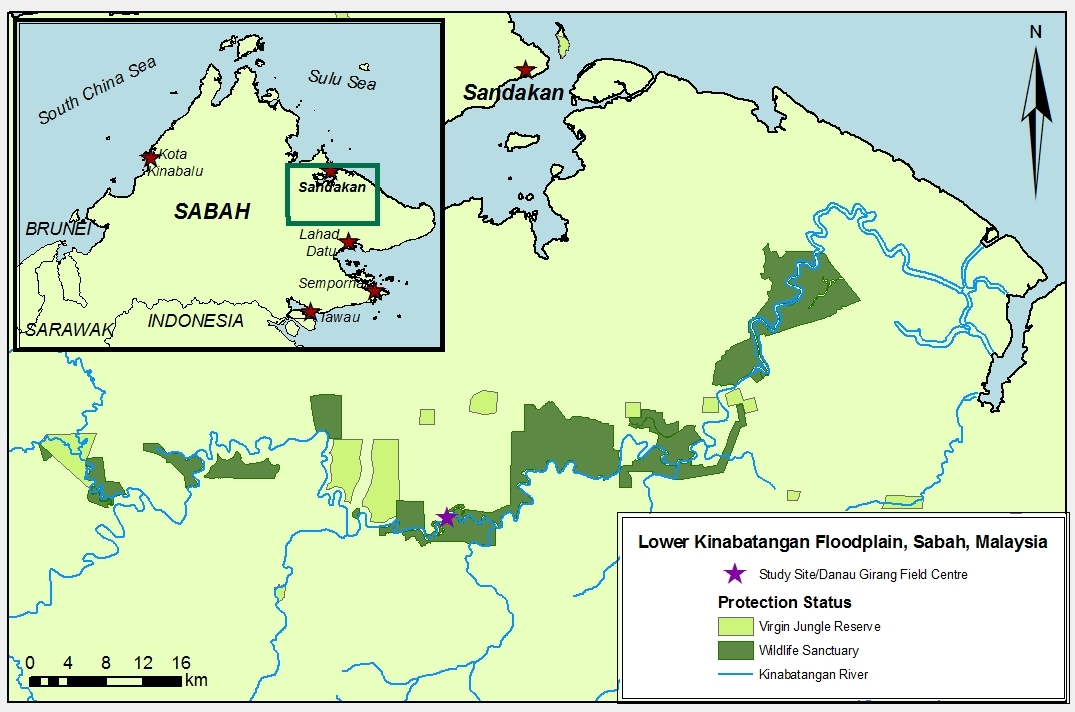
\includegraphics[width=\textwidth]{Chap3/figures/dgfc_map}
\caption{Map of Danau Girang in relation to Sabah Malaysia}
\label{int:fig:map}
\end{figure}

The Kinabatangan is a protected wildlife reserve, with thick and humid forest, making it very difficult to walk through and even more difficult for hardware to survive the conditions. Cameras are placed along the river and up to 1km into the forest, capturing images when triggered and saving them onto SD cards. These SD cards are collected and stored at the field centre, where the images are manually collated and processed. The cameras are designed to have a battery life of three months but, due to the humidity, a battery life of three weeks is more realistic. In 2010, twenty cameras were deployed and half of them were inspected every two weeks, on a rotating basis. In that time, each camera can record more than a thousand pictures and the dynamic nature of the rainforest, such as the sun through leaves, falling trees and reflections in the water can cause the camera to trigger when an animal has not walked past. The events are known as \textit{false triggers}, and they can make up to 70\% of the images on an SD card and each of these must be manually processed. 

Each trigger of the camera results in a set of three images being captured, this number has been chosen by the researchers at DGFC after some experimentation. Three images allows for more than one image of slow-moving animals to be captured and, typically, allows for the middle image in the sequence to capture the body of fast-moving animals; with the first and last capturing the head and rear respectively.

We have used this scenario to test our hypothesis and implement a WSN that automates the collection, transmission, processing and storage of images, using local knowledge to classify the data and prioritise the flow of information through the network, making more efficient use of the limited power and bandwidth available. 

\section{Research Contributions}

Here we outline the main research contributions explained in this thesis. We believe that two main contributions have been made and our experimental results serve to support these contributions.
Our primary contribution is that we propose a \textbf{novel tiered network architecture where each subsequent tier possesses increased knowledge-processing ability}, K-HAS, that utilises the local knowledge of its surrounding environment, users and previously sensed data to process observations within the network and prioritise the data according to the inferred classification. 

Knowledge is pushed out to the edge of the network to allow the nodes that capture observations to prioritise the data based on its content. The knowledge processing capabilities increase with each tier as the data moves toward the centre of the network, allowing more detailed inferences to be made and data to be given a higher priority. This smart utilisation of bandwidth allows data to be delivered in an order that is more useful than chronological, delivering the most valuable observations first and using human feedback to learn how important these observations were. 

In addition, K-HAS uses a feedback loop to dynamically update the knowledge base on every node throughout the deployment so it is able to react to changes within the data recorded, and the network, in near real-time.

Experimental results from the Malaysian rainforest showed that current long-range wireless sensor technology is not yet at the point where nodes could be deployed in a harsh environment and left without human intervention for months at a time. A modified K-HAS system LORIS (Local knowledge Remote-sensing Ontology-based Informatics System) combined tiers that use knowledge-processing at the centre of the network, with commercially available, wireless cameras. This showed that knowledge-processing automates the handling of sensed data when it is received and can be used to infer patterns for future observations. LORIS was designed because we could not find robust, open sensing nodes that can send data over long distances and handle high humidity and extreme temperatures. Because of this, we used off-the-shelf (OTS) wireless cameras that ran a closed system, while providing some access through proprietary software. We then combined two of K-HAS' tiers so that processing only took place at the base station, matching a more traditional WSN topology; while still making use of local knowledge gained from previously sensed data.

We model the ideal implementation of K-HAS in a simulation environment, along with variations on the knowledge processing capbilities of each node, We use these simulations to show that local and global knowledge can prioritise sensed data effectively and that this prioritisation increases the efficiency of the network by delivering data based on its importance, rather than chronologically.

Our second contribution is an \textbf{ontology that combines, and extends, ontologies used in multiple domains to create an extension ontology for WSNs and ecological observations}. To formally define the structure of K-HAS and the data standard used, we developed an ontology that combined existing ontologies for sensor networks and ecological observations. This ontology can be used as a whole or in parts for WSNs that use some, or all, of K-HAS' architecture. On top of this, we extended these ontologies by adding specific terms relevant to the different node types and users within the K-HAS architecture.

We apply this ontology to our proposed architecture, and simulations, in order to define a data standard for sensed data sent within the network, as well as terms to use in observations as well as identify the roles of both humans and sensors within the network.


\section{Thesis Structure}
The rest of this thesis is structured as follows. Chapter 2 provides background on wireless sensor networks and the use of knowledge-based technologies in that context. Chapter 3 explains technical decisions we made and the findings when running experiments in the Malaysian rainforest. Chapter 4 introduces the K-HAS architecture we have proposed and explains the purpose of each tier. Chapter 5 details the ontology we have proposed to support K-HAS and shows how current ontologies do not sufficiently cover all of the concepts involved with a \textit{scientific observation}. Chapter 6 details our implementation in the Malaysian Rainforest and the changes we had to make in order for it to be feasible. Chapter 7 describes how we modelled K-HAS, and other scenarios, in a simulation environment. The results are then explained and we explain how different scenarios are suited to WSNs, in a multitude of environments, with different requirements. Chapter 8 then concludes this thesis and summarises our contributions and findings, as well as highlighting work that could be undertaken to take this project further.
